\begin{appendix} 
\section{Galaxy properties and the \tttp covariance}
\label{app:properties}

This Appendix tabulates the properties of the KiDS-1000 tomographic source samples, along with the properties of the BOSS and 2dFLenS lens samples, in Table~\ref{tab:datatab}.   
We list the spectroscopic redshift selection for the lenses ($z_{\rm min} < z_{\rm s} \leq z_{\rm max}$), and the photometric redshift selection for the sources ($z_{\rm min} < z_{\rm B} \leq z_{\rm max}$), along with the mean redshift of each sample.  
For the source sample, the true redshift distributions are estimated in \citet{hildebrandt/etal:inprep}, using the SOM methodology from \citet{wright/etal:2020}.     
The shear calibration correction, $m$, which can also be referred to in the literature as the responsivity, $R = 1+m$, is listed for each source bin \citep{kannawadi/etal:2019}.  
The effective number density of lenses and sources defines the number of galaxies per square arcminute in the case of unit weights and, for the sources, unit responsivity \citep[see equations C.11 and C.13 in][]{joachimi/etal:inprep}.  
We also list the effective ellipticity dispersion, $\sigma_{\epsilon,i}$, per ellipticity component, $i$, for each the weighted and calibrated source galaxy samples \citep[equation C.8 in][]{joachimi/etal:inprep}.

\begin{table}
\caption{Galaxy properties for the BOSS and 2dFLenS lens (\lq L\rq) samples and the KiDS-1000 source (\lq S\rq) samples.}              % title of Table
\label{tab:datatab}      % is used to refer this table in the text
\centering                                      % used for centering table
\begin{tabular}{lcccccr}          % centered columns
\toprule
ID & $z_{\rm min}$ &  $z_{\rm max}$& mean $z$ & $n_{\rm eff}$ & $\sigma_{\epsilon,i}$ & \multicolumn{1}{c}{$m$}\\    % table heading
\midrule
\multicolumn{6}{l}{\bf KiDS-1000:}\\  
S1 & 0.1 & 0.3 & 0.26 & 0.62 &  0.27 & $-0.009\pm0.019$\\
S2 & 0.3 & 0.5 & 0.40 & 1.18 &  0.26 & $-0.011\pm0.020$\\
S3 & 0.5 & 0.7 & 0.56 & 1.85 &  0.27 & $-0.015\pm0.017$\\
S4 & 0.7 & 0.9 & 0.79 & 1.26 &  0.25 & $0.002\pm0.012$\\
S5 & 0.9 & 1.2 & 0.98 & 1.31 &  0.27 & $0.007\pm0.010$\\
\midrule      
\multicolumn{6}{l}{\bf BOSS:}\\                             % inserts single horizontal line
L1 & 0.2 & 0.5 & 0.38 & $0.014$ & -  & \multicolumn{1}{c}{-}\\
L2 & 0.5 & 0.75 & 0.61 & $0.016$ & -  & \multicolumn{1}{c}{-}\\
\midrule      
\multicolumn{6}{l}{\bf 2dFLenS:}\\                                % inserts single horizontal line
L1 & 0.2 & 0.5 & 0.36 & $0.006$ & - & \multicolumn{1}{c}{-}\\
L2 & 0.5 & 0.75 & 0.60 & $0.006$ & - & \multicolumn{1}{c}{-}\\
\bottomrule
\end{tabular}
\tablefoot{Columns include the bin identifier, ID, the minimum and maximum redshift selection for the bin, $z_{\rm min/max}$, which applies to photometric redshifts for the sources S, and spectroscopic redshifts for the lenses L, along with the mean redshift of the bin and the effective galaxy number density, per square arcminute, $n_{\rm eff}$.  For the source bins we also include the measured ellipticity dispersion per component, $\sigma_{\epsilon,i}$, and the shear calibration correction, $m$, and its uncertainty.}
\end{table}


Fig.~\ref{fig:ttttpcov} displays the correlation coefficients of the \tttp covariance matrix for the three observables; cosmic shear E-mode power spectra, $\mathcal{C}_E$, galaxy-galaxy lensing E-mode power spectra, $\mathcal{C}_{n\epsilon}$, and the anisotropic galaxy clustering in low and high redshift bins, $\xi_{\rm gg}$ (see Sect.~\ref{sec:data} for details).   The cross-correlation between the two lensing and the clustering observables is set to zero, as mock data analyses showed these correlations to be negligible for the KiDS and BOSS footprints \citep{joachimi/etal:inprep}.  The Fourier-space lensing observables are shown to be significantly less correlated between $\ell$-scales, in comparison to the physical-scale clustering observables.
\begin{figure}
	\begin{center}
		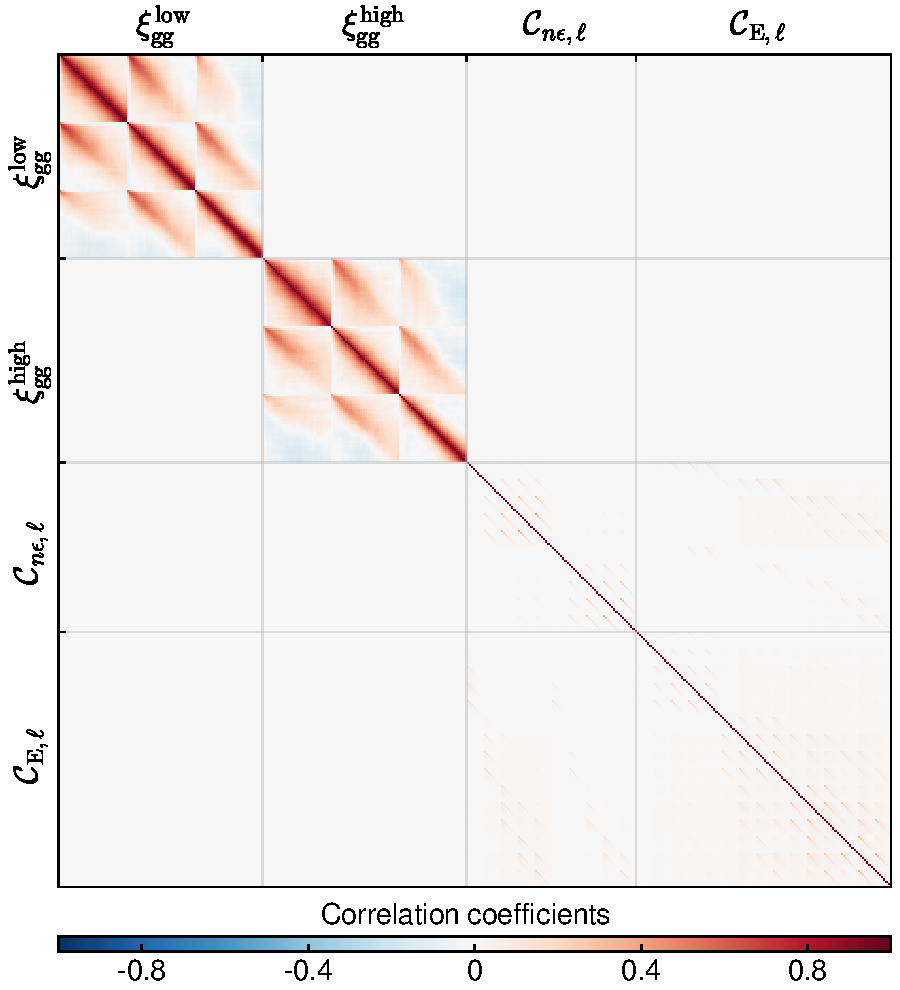
\includegraphics[width=\columnwidth]{Data_Plots/corr_paper_wedge+aPneE+aPeeE_obs_tot_theory}
		\caption{Correlation coefficients of the \tttp covariance matrix for the cosmic shear, $\mathcal{C}_{\rm E}$, galaxy-galaxy lensing, $\mathcal{C}_{n\epsilon}$ and galaxy clustering observables, $\xi_{\rm gg}$ (see Sect.~\ref{sec:data} for details).  Here the band powers $\mathcal{C}$, are related to the angular power spectrum $C$, in Eq.~(\ref{eq:cl_cosmicshear}) and Eq.~(\ref{eq:pgg}), as $\mathcal{C}= \ell^2 C/(2\pi)$.}
		\label{fig:ttttpcov}
	\end{center}
\end{figure}

\ch{
\section{Modelling Intrinsic Galaxy Alignment}
\label{app:IAmodel}
In this analysis we adopt the \citet{bridle/king:2007} NLA model in order to marginalise over our uncertainty in the contribution to the observed two-point shear correlation function from the intrinsic alignment (IA) of galaxies within their surrounding density field.   More sophisticated models exist, however, and in this appendix we briefly discuss these alternatives.   We then provide justification for our choice by summarising the analysis of \citet{fortuna/etal:2020} which demonstrates that for the statistical power of KiDS-1000, the use of the somewhat adhoc NLA model is sufficiently flexible so as not to introduce any biases in the cosmological parameter constraints.

There are two advanced approaches to determine a non-linear IA model.    The first uses a perturbative approach to model the non-linear behaviour of the tidal alignment (where the galaxy is preferentially aligned with the `stretching axis' of the tidal quadrupole) and tidal torquing (where the galaxy disc forms perpendicular to the angular momentum axis which is dependent on the tidal field) \citep{blazek/etal:2019, vlah/etal:2020}.  The second uses a halo model approach, which introduces a model for the small-scale alignment of satellite galaxies within central haloes \citep{schneider/bridle:2010}, and allows for different alignment strengths to be included for the evolving red and blue galaxy population \citep{fortuna/etal:2020}.  On large physical scales both approaches, along with the NLA model, recover the linear alignment model of \citet{hirata/seljak:2004}.  On small physical scales the accuracy of the perturbative approach is limited by the order of the corrections adopted \citep{blas/etal:2013}.  The accuracy of the halo model approach is limited by the challenge of modelling the transition between the properties of galaxies within single halos and the across full density field, commonly referred to as the one-to-two halo transition \citep[see for example the discussion in][]{mead/etal:2020b}.   Both models are nevertheless a significant improvement on the NLA model, which developed an adhoc solution to a small-scale mismatch of the \citet{hirata/seljak:2004} model with IA numerical simulations \citep{heymans/etal:2004}, by replacing the linear matter power spectrum in the \citet{hirata/seljak:2004} formalism with the non-linear matter power spectrum.

IA observations of red and blue galaxies have been both direct \citep{joachimi/etal:2011,mandelbaum/etal:2011,singh/etal:2015,tonegawa/etal:2018,johnston/etal:2019} and indirect \citep{heymans/etal:2013, samuroff/etal:2019}, recovering a common conclusion of significant alignment for red galaxies, and, as yet, no detection of alignment for blue galaxies.   Direct observations are limited by the depth of the spectroscopic galaxy samples that can be studied.  Indirect observations, where an IA model is constrained simultaneously with a cosmological model, are limited by degeneracies with nuisance parameters.   As the IA and cosmological signal scale differently with redshift, a flexible IA model can absorb any systematic errors in the shape of the source redshift distributions, such that the resulting IA parameter constraints are not a true reflection of the underlying IA  model.    This point is nicely illustrated in figure 5 of \citet{efstathiou/lemos:2018} where indirect constraints on the amplitude of the NLA model for the full galaxy sample are shown to vary from $ -6 < A_{\rm IA} < 6$ across a wide range of published cosmic shear surveys.  \citet{wright/etal:2020b} present another example, analysing mock galaxy catalogues to improve the accuracy of the priors on the redshift uncertainty for the previous KiDS data release.  In this case the fiducial IA constraint $A_{\rm IA} = 0.95 \pm 0.67$ reduces to $A_{\rm IA} = 0.28 \pm 0.59$ with the inclusion of a more accurate redshift uncertainty model.   As the intrinsic alignment model depends on the cosmology, any tendency for the model to incorrectly absorb redshift errors would inadvertently lead to unexpected biases in the cosmological parameter constraints.   The more freedom afforded to the IA model, the more opportunity there is for such biases to occur.    Given this concern, we choose to adopt the minimal IA model freedom afforded by current direct observational IA constraints.  In this way any unaccounted errors in our redshift distributions can be detected through a poor goodness-of-fit of the combined cosmological and IA model, as seen, for our second tomographic redshift bin, in the KiDS-1000 internal consistency analysis of \citet[][appendix B.2]{asgari/etal:2020}.   


Our choice of the one-parameter NLA model is motivated by the IA halo model analysis of \citet{fortuna/etal:2020}.   In this analysis central red galaxies are modelled using the  \citet{hirata/seljak:2004} model, with an amplitude $A_{\rm red}$ and a luminosity dependent scaling $\propto L^\beta$.   Combining the observed constraints from \citet{joachimi/etal:2011, singh/etal:2015} they model a simple power-law scaling model with $A_{\rm red} = 5.3 \pm 0.6$ and $\beta=1.2 \pm 0.4$.   The additional constraints from \citet{johnston/etal:2019} motivate a broken power-law model with $A_{\rm red} = 5.1 \pm 1.0$ and $\beta_{L \geq L_0}=1.2 \pm 0.4$, which they also consider.    Central blue galaxies follow the \citet{hirata/seljak:2004} model, with a \citet{johnston/etal:2019} constrained amplitude of $A_{\rm blue} = 0.2 \pm 0.4$ and no luminosity dependence, as there is no observational evidence to support this.    The satellite galaxy alignments are modelled following \citet{schneider/bridle:2010}.  The amplitude, radial and luminosity dependence of the alignment of red and blue satellite galaxies within their host halo is independently constrained following \citet{georgiou/etal:2019}.     

The direct IA observational constraints adopted by \citet{fortuna/etal:2020} are determined from low redshift galaxy samples, where the properties of the full galaxy population differ significantly from the high redshift galaxy population analysed in KiDS-1000.  Given that the fundamental physical processes that underpin the intrinsic alignment mechanisms are unlikely to evolve, however, these galaxy-type-specific constraints are relevant at all redshifts, provided the evolution in the relative fractions, luminosities and distribution of the red and blue, central and satellite, galaxy populations are accurately modelled.   

\citet{fortuna/etal:2020} determine a sample of plausible IA models for a KiDS-like survey.  They combine the different galaxy-type IA contributions using a halo occupation distribution model taken from the MICE mock galaxy catalogues \citep{fosalba/etal:2015}, with a magnitude limit corresponding to KiDS-depth.   The range of full-population models encompasses the observational uncertainty on the IA model parameters for each galaxy type.    Analysing these IA halo-models with the NLA model, they find the highest NLA model amplitude of $A_{\rm IA}=0.54 \pm 0.13$ when adopting a broken power-law for the red-central luminosity scaling.    This is fully consistent with the \citet{asgari/etal:2020} KiDS-1000 COSEBIs cosmic shear constraints with $A_{\rm IA}=0.26 ^{+0.42}_{-0.34}$, the KiDS-1000 band power cosmic shear constraints with $A_{\rm IA}=0.97 ^{+0.29}_{-0.38}$ and the KiDS-1000 \tttp band power constraints with $A_{\rm IA}=1.07^{+0.27}_{-0.31}$, with the largest difference found for the \tttp results which are in 1.6$\sigma$ agreement.    

Adopting the NLA model in a cosmological parameter inference of a mock KiDS-like data vector of the cosmic shear signal contaminated by the range of different IA halo models allowed by observations, \citet{fortuna/etal:2020} conclude that the redshift dependence of the true IA halo model is not large enough to bias the cosmological parameters in a KiDS-like cosmic shear analysis with the NLA model.   \citet{asgari/etal:2020} nevertheless explore one extension of the NLA model, with the inclusion of a redshift-dependent scaling term, which does not change the recovered KiDS-1000 cosmic shear MAP $S_8$ value, and only serves to increase the marginal credible region of $S_8$ by $\sim 10\%$.   For these reasons, we adopt a minimal one-parameter NLA model in our \tttp analysis, but recognise that in future surveys such as LSST and {\it Euclid}, this adhoc model will no longer be sufficient given the expected statistical power of these next-generation surveys \citep{blazek/etal:2019, fortuna/etal:2020}.

}

\section{Parameter priors}
\label{app:priors}
This Appendix tabulates the adopted KiDS-1000 priors and sampling parameters in Table~\ref{tab:priors}.   
The uniform prior on the dimensionless Hubble constant, $h$, reflects distance-ladder $\pm 5\,\sigma$ constraints from \citet{riess/etal:2016}, which encompasses the value of $h$ favoured by \citet{planck/etal:2018}.  
The uniform prior on the baryon density, $\omega_{\rm b}= \Omega_{\rm b}h^2$, reflects big bang nucleosynthesis $\pm 5\, \sigma$ constraints from \citet{olive/etal:2014}.   
The uniform prior on the CDM density, $\omega_{\rm c} = \Omega_{\rm c}h^2$, reflects Supernova Type Ia $\pm 5\, \sigma$ constraints on $\Omega_{\rm m}$ from \citet{scolnic/etal:2018} combined with the most extreme allowed values of $h$ and $\omega_{\rm b}$, given their priors.   

As discussed in Sect.~\ref{sec:KCAP} we choose to sample with an uninformative uniform prior on $S_8$ to avoid implicit informative priors from a uniform prior on the primordial power spectrum amplitude $A_{\rm s}$.    
We choose a fixed model for the properties of neutrinos, adopting the normal hierarchy at the minimum sum of masses, $\Sigma m_\nu = 0.06\,\mathrm{eV}$, following \citet{planck/etal:2018}.  
We consider extended models, including variations on neutrino mass in \citet{troester/etal:inprep}.

\begin{table}
\caption{KiDS-1000 sampling parameters and priors.}              % title of Table
\label{tab:priors}      % is used to refer this table in the text
\centering                                      % used for centering table
\begin{tabular}{lll}          % centered columns (4 columns)
\toprule
Parameter & Symbol & Prior \\    % table heading
\midrule                                   % inserts single horizontal line
Hubble constant & $h$ & $\bb{0.64,\,0.82}$ \\
Baryon density & $\omega_{\rm b}$ & $\bb{0.019,\,0.026}$ \\
CDM density & $\omega_{\rm c}$ & $\bb{0.051,\,0.255}$ \\
Density fluctuation amp. & $S_8$ & $\bb{0.1,\,1.3}$ \\
Scalar spectral index & $n_{\rm s}$ & $\bb{0.84,\,1.1}$ \\
\midrule
Linear galaxy bias & $b_1 \;[2]$ & $\bb{0.5,\,9}$ \\
Quadratic galaxy bias & $b_2 \;[2]$ & $\bb{-4,\,8}$ \\
Non-local galaxy bias & ${\gamma_3^-} \;[2]$ & $\bb{-8,\,8}$ \\
Virial velocity parameter & $a_{\rm vir} \;[2]$ & $\bb{0,\,12}$ \\
Intrinsic alignment amp. & $A_{\rm IA}$ & $\bb{-6,\,6}$ \\
Baryon feedback amp. & $A_{\rm bary}$ & $\bb{2,\,3.13}$ \\
\midrule
Redshift offsets & ${\bf \delta_z}$ & ${\cal N}(\vek{\mu};\vek{C}_{\delta z})$ \\
\bottomrule
\end{tabular}
\tablefoot{Primary cosmological parameters for the flat $\Lambda$CDM model are listed in the first section. The second section lists astrophysical nuisance parameters to model galaxy bias (with independent parameters for each of the two BOSS redshift bins as indicated with the bracket $[2]$), intrinsic galaxy alignments, and baryon feedback.  Observational redshift nuisance parameters are listed in the final section. Prior values in square brackets are the limits of the adopted uniform top-hat priors.  ${\cal N}(\mu;C)$ corresponds to a five dimensional multivariate Gaussian prior with mean $\vek{\mu}$ and covariance $\vek{C}_{\delta z}$.}
\end{table}

The uniform prior on the scalar spectral index, $n_{\rm s}$, reflects a restriction in our likelihood implementation, where the \citet{sanchez/etal:2017} galaxy clustering likelihood becomes prohibitively slow for $n_{\rm s}>1.1$.  With the upper limit of the top-hat prior fixed by this computational limitation, we choose to symmetrise the prior around the theoretical expectation of $n_{\rm s}=0.97$.     In Fig.~\ref{fig:ns-prior} we demonstrate the impact of this informative prior on the BOSS-only galaxy clustering constraints, highlighting how informative this choice of prior is.   We argue that adopting an informative prior is justified however, given our theoretical prior knowledge of the Harrison-Zel'dovich spectrum.   Fig.~\ref{fig:ns-prior} also helps to illustrate that had we chosen an uninformative prior on $n_{\rm s}$ for our KiDS-1000-BOSS analysis, a decision taken more than a year before unblinding our analysis, this would have likely served to exacerbate any tension with the Planck CMB constraints. 

\begin{figure}
	\begin{center}
		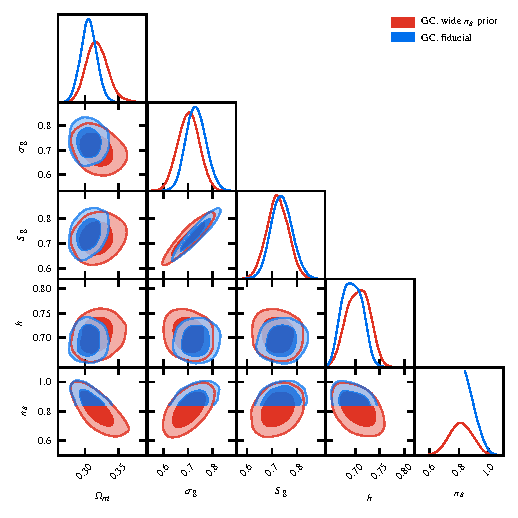
\includegraphics[width=\columnwidth]{Parameter_Plots/systematics/GC_ns_prior}
		\caption{The impact of the $n_{\rm s}$ prior: Comparing marginalised posterior distributions for the BOSS galaxy clustering analysis for our fiducial analysis (blue) with the constraints when adopting an uninformative prior on $n_{\rm s}$ (orange).   Opening the parameter space to arguably unphysical values of $n_{\rm s}$ favours higher values and weaker constraints on $\Omega_{\rm m}$. Constraints on $S_8$ are, however, fairly insensitive to the choice of $n_{\rm s}$ prior.}
		\label{fig:ns-prior}
	\end{center}
\end{figure}

Turning to astrophysical priors, the galaxy bias parameter top-hat priors on $b_1$, $b_2$,  $\gamma_3^-$, (Eq.~\ref{eq:pgg}), and on $a_{\rm vir}$ \citep[see the `fingers of god' model in equations 6 to 9 of][]{joachimi/etal:inprep},
match those adopted in \citet{troester/etal:2020}, which cover a wider range than those used in \citet{sanchez/etal:2017}.  
The two BOSS redshift slices have independent sets of parameters.   
Wide uniform priors for the intrinsic alignment parameter $A_{\rm IA}$ are chosen to be uninformative.    
Uniform priors on the baryon feedback parameter $A_{\rm bary}$ are chosen such that the resulting \citet{mead/etal:2015} model of the non-linear matter power spectrum encompasses both the most aggressive feedback model from the \citet{vandaalen/etal:2011} suite of hydrodynamical simulations, along with the dark matter-only case where $A_{\rm bary}=3.13$.

There are five additional correlated nuisance parameters, $\delta^i_z$, that model uncertainty in the mean of the source redshift distributions.  We adopt a multivariate Gaussian prior for the vector $\vek{\delta}_z$ with a mean $\vek{\mu} = (0.0001,0.0021,0.0129,0.0110,-0.0060)$, and a covariance, $C_{\delta z}$, as calibrated using mock galaxy catalogues in \citet{wright/etal:2020}.   
The diagonal terms of $\vek{C}_{\delta z}$ are typically at the level of $\sim\!(0.01)^2$, with off-diagonal correlation coefficients ranging between $\sim\! 0.1$ and $\sim\! 0.3$ \citep[see section 3 and figure 2 of][for details]{hildebrandt/etal:inprep}.


\section{Parameter constraints}
\label{app:parameter-constraints}
This Appendix tabulates the maximum posterior (MAP) and marginalised constraints on the flat $\Lambda$CDM cosmological parameters, in Table~\ref{tab:fullparams}, for the different combinations of the three large-scale structure probes considered in this work.   For constraints from KiDS-1000 cosmic shear alone, we refer the reader to \citet{asgari/etal:inprep}.
\begin{landscape}
\begin{table}
\begin{center}
\caption{Parameter constraints for the probe combinations considered in this work: \tttp, cosmic shear (CS) and galaxy-galaxy lensing (GGL), cosmic shear and galaxy clustering (GC), and galaxy clustering by itself. 
We refer the reader to \citet{asgari/etal:inprep} for cosmic shear-only constraints. 
For each probe, the first column lists the MAP value with the PJ-HPD CI. 
If the PJ-HPD CI could not be robustly determined, no uncertainty estimate is provided. 
The second column for each probe lists the maximum of the marginal posterior, together with the marginal HPD CI. 
Parameter for which the marginal probability at either prior edge exceeds 13\% of the peak probability are deemed unconstrained and are denoted by a dash. 
Finally, parameters that are not sampled are left blank.
\label{tab:fullparams}}
\begin{tabular}{lllllllll}
    \toprule
    Parameter    & $3\times2$pt & $3\times2$pt& GC & GC& CS+GGL & CS+GGL& CS+GC & CS+GC \\ 
             & (joint) & (marginal)& (joint) & (marginal)& (joint) & (marginal)& (joint) & (marginal) \\ 

    \midrule
$S_8     $& $0.766^{+0.02}_{-0.014}$ & $0.765^{+0.017}_{-0.016}$& $0.762^{+0.054}_{-0.05}$ & $0.743^{+0.038}_{-0.05}$& $0.774^{+0.031}_{-0.029}$ & $0.761^{+0.024}_{-0.025}$& $0.766^{+0.018}_{-0.015}$ & $0.763^{+0.016}_{-0.016}$\\ [0.3 em]
$h^2\Omega_\mathrm{c}$& $0.123$ & $0.124^{+0.0096}_{-0.011}$& $0.136^{+0.0065}_{-0.018}$ & $0.123^{+0.011}_{-0.009}$& $0.0721^{+0.089}_{-0.016}$ & $0.12^{+0.057}_{-0.034}$& $0.126^{+0.0075}_{-0.013}$ & $0.124^{+0.01}_{-0.011}$\\ [0.3 em]
$h^2\Omega_\mathrm{b}$& $0.0225$ & --& $0.0246^{+0.0012}_{-0.0037}$ & --& $0.0258$ & --& $0.0219^{+0.0022}_{-0.0022}$ & --\\ [0.3 em]
$h       $& $0.695^{+0.03}_{-0.019}$ & $0.696^{+0.02}_{-0.026}$& $0.716^{+0.02}_{-0.035}$ & $0.687^{+0.029}_{-0.018}$& $0.642^{+0.1}_{-1.2e-05}$ & --& $0.695^{+0.022}_{-0.023}$ & $0.69^{+0.026}_{-0.02}$\\ [0.3 em]
$n_\mathrm{s}$& $0.901$ & --& $0.851^{+0.06}_{-0.01}$ & --& $0.947$ & --& $0.894^{+0.05}_{-0.042}$ & --\\ [0.3 em]
\midrule
$A_{\rm bary}$& $3.13^{+1.6e-05}_{-0.47}$ & --& $$ & & $3.13$ & --& $3.13$ & --\\ [0.3 em]
$A_{\rm IA}$& $1.07^{+0.27}_{-0.31}$ & $1.01^{+0.31}_{-0.28}$& $$ & & $0.974^{+0.32}_{-0.2}$ & $0.972^{+0.25}_{-0.26}$& $0.947^{+0.44}_{-0.31}$ & $0.892^{+0.35}_{-0.36}$\\ [0.3 em]
$\delta \bar{z_1}$& $1.93^{+11}_{-10}\times 10^{-3}$ & $2.8^{+8.8}_{-12}\times 10^{-3}$& $$ & & $1.41^{+8.4}_{-11}\times 10^{-3}$ & $2.15^{+8.7}_{-11}\times 10^{-3}$& $2.02^{+7.4}_{-14}\times 10^{-3}$ & $2.45^{+9.5}_{-12}\times 10^{-3}$\\ [0.3 em]
$\delta \bar{z_2}$& $0.0101^{+0.016}_{-0.0068}$ & $9.09^{+-9.1}_{-9.1}$& $$ & & $0.0102^{+0.014}_{-0.0069}$ & $8.75^{+-8.7}_{-8.8}$& $0.0117^{+0.013}_{-0.0085}$ & $0.0121^{+0.0095}_{-0.012}$\\ [0.3 em]
$\delta \bar{z_3}$& $-0.0207^{+0.0093}_{-0.01}$ & $-0.0204^{+0.01}_{-0.0093}$& $$ & & $-0.0206^{+0.0091}_{-0.0091}$ & $-0.0199^{+0.0092}_{-0.0092}$& $-0.013^{+0.0091}_{-0.012}$ & $-0.0119^{+0.0098}_{-0.011}$\\ [0.3 em]
$\delta \bar{z_4}$& $-0.0143^{+0.0076}_{-0.008}$ & $-0.0145^{+0.0082}_{-0.0076}$& $$ & & $-0.0138^{+0.0066}_{-0.0086}$ & $-0.012^{+0.0062}_{-0.009}$& $-0.0166^{+0.0098}_{-0.0064}$ & $-0.0156^{+0.0077}_{-0.0085}$\\ [0.3 em]
$\delta \bar{z_5}$& $5.23^{+8.3}_{-10}\times 10^{-3}$ & $4.54^{+10}_{-8.7}\times 10^{-3}$& $$ & & $6.06^{+7.3}_{-10}\times 10^{-3}$ & $6.85^{+8.7}_{-8.6}\times 10^{-3}$& $6.5^{+12}_{-7.1}\times 10^{-3}$ & $6.54^{+9.4}_{-9}\times 10^{-3}$\\ [0.3 em]
$b_1^{\rm lowz}$& $2^{+0.079}_{-0.083}$ & $2.04^{+0.064}_{-0.093}$& $2.01^{+0.13}_{-0.16}$ & $2.09^{+0.11}_{-0.13}$& $3.29^{+0.3}_{-0.81}$ & $3.14^{+0.55}_{-0.55}$& $1.99^{+0.09}_{-0.07}$ & $2.02^{+0.085}_{-0.07}$\\ [0.3 em]
$b_2^{\rm lowz}$& $0.3^{+0.62}_{-0.69}$ & $0.289^{+0.71}_{-0.61}$& $0.475^{+1.1}_{-0.83}$ & $0.624^{+0.96}_{-1}$& $0.968$ & --& $0.443^{+1}_{-0.67}$ & $0.326^{+1}_{-0.67}$\\ [0.3 em]
$\gamma_{3-}^{\rm lowz}$& $0.695^{+0.48}_{-0.54}$ & $0.879^{+0.44}_{-0.52}$& $0.688^{+0.59}_{-0.57}$ & $0.752^{+0.62}_{-0.56}$& $7.87$ & --& $0.594^{+0.58}_{-0.57}$ & $0.853^{+0.53}_{-0.52}$\\ [0.3 em]
$a_{\rm vir}^{\rm lowz}$& $4.14^{+0.84}_{-0.97}$ & $4.24^{+0.86}_{-0.96}$& $4.3^{+1.1}_{-1.2}$ & $4.44^{+1.1}_{-1.2}$& $$ & & $4.28^{+1.2}_{-1}$ & $4.37^{+1.1}_{-1.1}$\\ [0.3 em]
$b_1^{\rm highz}$& $2.13^{+0.095}_{-0.091}$ & $2.17^{+0.083}_{-0.093}$& $2.14^{+0.16}_{-0.16}$ & $2.23^{+0.13}_{-0.14}$& $2.3^{+0.33}_{-0.68}$ & $2.26^{+0.48}_{-0.52}$& $2.12^{+0.1}_{-0.094}$ & $2.17^{+0.092}_{-0.084}$\\ [0.3 em]
$b_2^{\rm highz}$& $-1.15^{+0.75}_{-0.41}$ & $-1.03^{+0.72}_{-0.46}$& $-0.948^{+2.3}_{-0.75}$ & $-0.901^{+2.3}_{-1}$& $5.82^{+2}_{-3.2}$ & --& $-1.16^{+1.8}_{-0.48}$ & $-0.951^{+1.7}_{-0.85}$\\ [0.3 em]
$\gamma_{3-}^{\rm highz}$& $0.369^{+0.8}_{-0.79}$ & $0.505^{+0.9}_{-0.62}$& $-0.126^{+0.94}_{-1.1}$ & $0.452^{+0.7}_{-1.2}$& $8^{+0.00058}_{-5.4}$ & --& $-0.0141^{+0.91}_{-0.91}$ & $0.412^{+0.8}_{-0.81}$\\ [0.3 em]
$a_{\rm vir}^{\rm highz}$& $1.18^{+1.5}_{-0.97}$ & --& $1.84^{+2.4}_{-1.8}$ & --& $$ & & $1.32^{+2.7}_{-1.3}$ & --\\ [0.3 em]
\midrule
$\Omega_\mathrm{m}$& $0.305^{+0.01}_{-0.015}$ & $0.306^{+0.012}_{-0.013}$& $0.313^{+0.0097}_{-0.017}$ & $0.307^{+0.011}_{-0.015}$& $0.239^{+0.11}_{-0.076}$ & $0.29^{+0.087}_{-0.07}$& $0.306^{+0.013}_{-0.012}$ & $0.307^{+0.012}_{-0.014}$\\ [0.3 em]
$\sigma_8$& $0.76^{+0.025}_{-0.02}$ & $0.759^{+0.02}_{-0.024}$& $0.75^{+0.045}_{-0.047}$ & $0.725^{+0.048}_{-0.036}$& $0.867^{+0.2}_{-0.17}$ & $0.729^{+0.13}_{-0.098}$& $0.758^{+0.028}_{-0.018}$ & $0.758^{+0.019}_{-0.024}$\\ [0.3 em]
$\sigma_{12}$& $0.743^{+0.03}_{-0.026}$ & $0.737^{+0.029}_{-0.027}$& $0.717^{+0.058}_{-0.035}$ & $0.707^{+0.046}_{-0.04}$& $0.887^{+0.15}_{-0.23}$ & $0.72^{+0.095}_{-0.14}$& $0.734$ & $0.732^{+0.03}_{-0.024}$\\ [0.3 em]
$S_{12}  $& $0.754^{+0.021}_{-0.013}$ & $0.754^{+0.015}_{-0.018}$& $0.751^{+0.038}_{-0.054}$ & $0.728^{+0.041}_{-0.045}$& $0.77^{+0.067}_{-0.046}$ & $0.757^{+0.036}_{-0.05}$& $0.753^{+0.022}_{-0.013}$ & $0.754^{+0.014}_{-0.019}$\\ [0.3 em]
$A_\mathrm{s}$& $1.85^{+0.25}_{-0.17}\times 10^{-9}$ & $1.79^{+0.22}_{-0.18}\times 10^{-9}$& $1.7^{+0.33}_{-0.16}\times 10^{-9}$ & $1.64^{+0.27}_{-0.18}\times 10^{-9}$& $5.34^{+5.2}_{-4.3}\times 10^{-9}$ & --& $1.81^{+0.27}_{-0.15}\times 10^{-9}$ & $1.78^{+0.21}_{-0.18}\times 10^{-9}$\\ [0.3 em]
$100\theta_{\rm MC}$& $1.05$ & $1.05^{+0.011}_{-0.015}$& $1.06^{+0.0082}_{-0.019}$ & $1.05^{+0.012}_{-0.013}$& $0.96^{+0.13}_{-0.023}$ & $1.09^{+0.039}_{-0.058}$& $1.05^{+0.009}_{-0.016}$ & $1.05^{+0.012}_{-0.014}$\\ [0.3 em]
    \bottomrule
\end{tabular}


\end{center}
\end{table}
\end{landscape}


\section{Sensitivity tests}
\label{app:sensitivity}

\begin{figure*}
	\begin{center}
		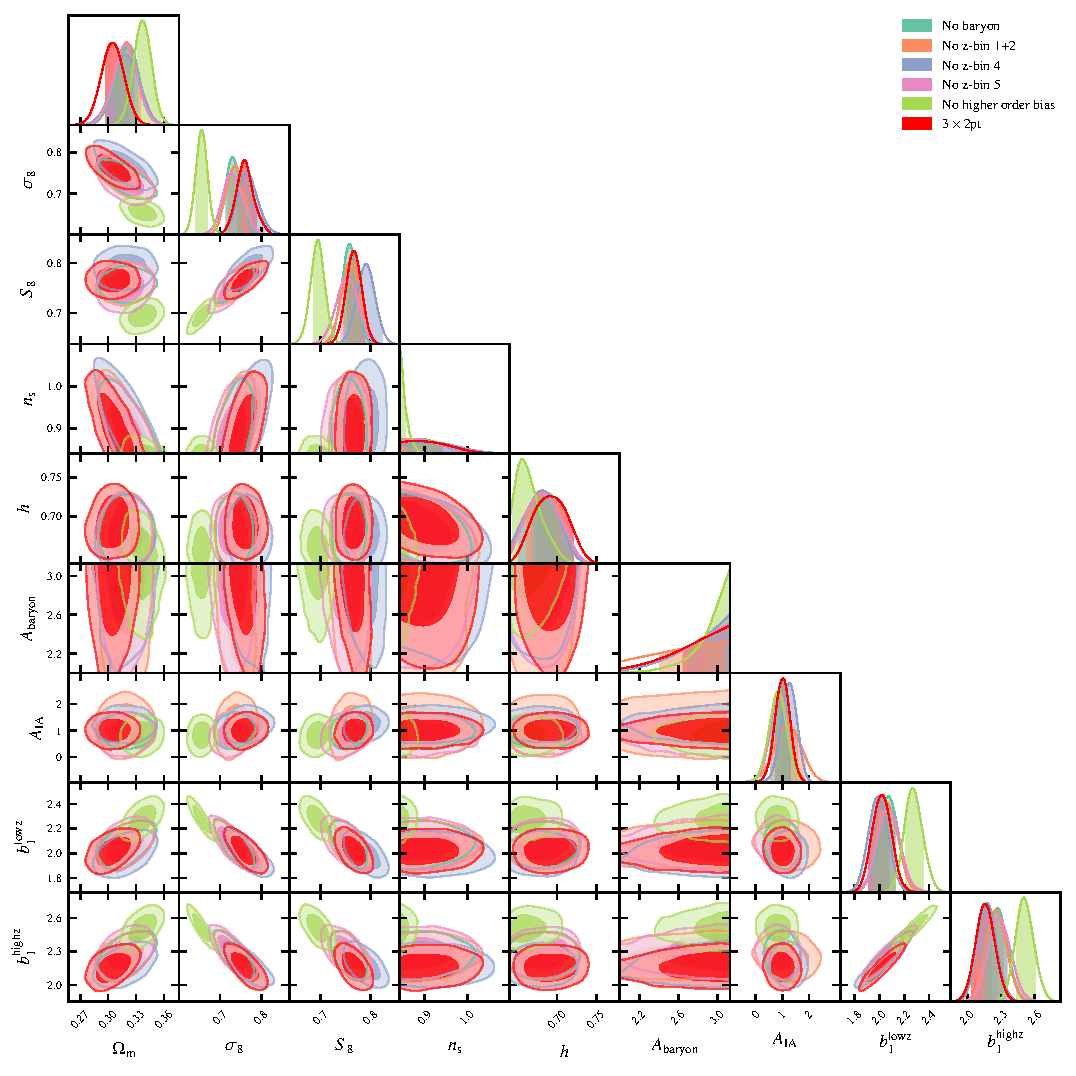
\includegraphics[width=\textwidth]{Parameter_Plots/systematics/blind_C_EE_nE_w_systematics_chains}
		\caption{Marginalised posterior distributions for the extended set of cosmological parameters shown in Fig.~\ref{fig:cosmology-params-all}, comparing the fiducial \tttp analysis (red) to a selection of our sensitivity test analyses where we ignore the impact of baryon feedback (the `No baryon' case, sea-green), limit the analysis to a linear galaxy bias model (the `No higher order GC' case, lime-green), and remove individual tomographic bins from our weak lensing observables (orange, purple and pink).}
		\label{fig:sensitivity_tests}
	\end{center}
\end{figure*}

In this Appendix we present, with Fig.~\ref{fig:sensitivity_tests}, the marginalised posterior distributions for a selection of the \tttp sensitivity tests explored in Sect.~\ref{sec:results}.  
These tests were all shown to recover consistent constraints on $S_8$, in Fig.~\ref{fig:S8comp}.  Here we explore these tests in more detail.    

We compare our analysis which fully marginalises over our uncertainty in the baryon feedback parameter (red), with our `No baryon' case (sea-green), where $A_{\rm bary}=3.13$, corresponding to the non-linear matter power spectrum for a dark-matter only cosmology.   
Here we find very little difference, as our \tttp analysis already favours high values of $A_{\rm bary}$.   
Our choice of scales and adoption of the band-power cosmic shear statistic for this analysis also makes us less sensitive to uncertainties in the baryon feedback parameter, compared to a standard two-point correlation function analysis \citep{asgari/etal:2020_KD}.

The removal of the two highest photometric redshift bins (blue and purple) primarily impacts $S_8$.   
These two bins carry the majority of the signal-to-noise in our analysis, and so it is not surprising that the removal of nearly half the constraining data, in each case, can result in $\sim\! 1\,\sigma$ changes in the recovered $S_8$ (see for example the discussion in Appendix~\ref{app:expectedoffsets}).   
We refer the reader to \citet{asgari/etal:inprep} where we present a detailed internal consistency analysis of the cosmic shear signal, following \citet{kohlinger/etal:2019}, \citep[see also][]{efstathiou/lemos:2018},  concluding that the two highest photometric redshift bins are consistent with the full data set.   
A potential $\sim\! 3\,\sigma$-level flag is, however, raised in \citet{asgari/etal:inprep}, 
over the internal consistency of the second tomographic bin.  
In our analysis where we remove the two lowest photometric redshift bins (orange), we find that these bins contribute very little to the $S_8$ constraint, and only serve to tighten the constraints on the intrinsic alignment parameter $A_{\rm IA}$.

Finally we turn to the galaxy bias test (lime green), where we limit the analysis to a linear galaxy bias model, $b_1$, setting all higher-order bias terms in Eq. (\ref{eq:pgg}) to zero\footnote{Removing all higher-order galaxy bias terms also requires the uncoupling of $b_1$ from $\gamma_2$.}, as well as imposing a Gaussian galaxy velocity distribution by setting $a_{\rm vir}$ to zero.   
We can see that this biases the recovered cosmological constraints, as the amplitude of the linear galaxy bias increases in an attempt to model the enhanced power on small scales that the non-linear bias induces.   
The erroneous increase in $b_1$ leads to a decrease in the recovered $S_8$, and also an overall reduction in the goodness-of-fit of the model with $\chi^2_{\rm MAP} = 379.8$ for $\sim\! 300$ degrees of freedom.  This result should serve as a point of caution for \tttp analyses that adopt an effective linear bias model \citep[see also the discussion in][]{asgari/etal:2020}, although we note that our analysis is particularly sensitive to the galaxy bias model given the high signal-to-noise BOSS clustering observations that probe physical scales as low as $s_{\rm min}= 20 h^{-1}\, {\rm Mpc}$.

\section{Expected $S_8$ differences between partially overlapping weak lensing surveys}
\label{app:expectedoffsets}
In this Appendix we construct a simple model to estimate the expected statistical fluctuation in $S_8$ constraints from partially overlapping weak lensing surveys, specifically our previous \citep[KV450,][]{wright/etal:2020b}, and current KiDS analyses.   Assuming that we only wish to constrain the overall amplitude of the measurement, the inference can be approximated by a linear least-squares problem, where $S_{8}$, the parameter of interest, is Gaussian distributed. 

In the following, measurements derived from the KV450 footprint are denoted by an $X$ in the subscript, while measurements on the new area added for KiDS-1000 are denoted with a $Y$. 
Measurements derived from the full KiDS-1000 footprint are denoted with a $Z$. 
Now, let $S^{\rm KV450}_{X}$ denote the value of $S_{8}$ estimated from the KV450 footprint, using the KV450 methodology; $S^\text{KiDS-1000}_{Y}$ the value estimated from the newly added area using the KiDS-1000 methodology; and $S^\text{KiDS-1000}_{Z}$ the KiDS-1000 value estimated from the full footprint. 
Approximating the estimates from disjoint footprints as independent, the $S_8$ measurement from the full KiDS-1000 area is then given by the area-weighted average\footnote{The amplitude of the weak lensing signal scales roughly with $S_8$ \citep{jain/seljak:1997}, with an uncertainty variance that scales with the inverse survey area \citep{schneider/etal:2002}.}
\begin{equation}
  S^\text{KiDS-1000}_Z = \frac{A_X S^\text{KiDS-1000}_X + A_Y S^\text{KiDS-1000}_Y}{A_Z} \, .
\end{equation}
Here $A_X$ is the effective area of the KV450 footprint, $A_Z$ is the effective area of the KiDS-1000 footprint, and $A_Y = A_Z - A_X$, is the additional area added between the two data releases.  
The uncertainty $\sigma_{X}^\text{KiDS-1000}$ on the measurement $S^\text{KiDS-1000}_X$ is then related to the uncertainty $\sigma_Z^\text{KiDS-1000}$ on measurements $S^\text{KiDS-1000}_Z$, as 
\be
\sigma_{X}^\text{KiDS-1000} = \sqrt{\frac{A_Z}{A_X}}\, \sigma_Z^\text{KiDS-1000} \, ,
\ee
and analogously for $\sigma_{Y}^\text{KiDS-1000}$. 
Note that the uncertainty $\sigma^{\rm KV450}_{X}$ differs from $\sigma_{X}^\text{KiDS-1000}$ due to differences in the KiDS-1000 and KV450 methodologies, such as the adopted $m$-calibration uncertainty. 

We define $\Delta = S^\text{KiDS-1000}_Z - S^{\rm KV450}_X$, the offset between the KiDS-1000 and KV450 $S_{8}$ measurements.  
The uncertainty on $\Delta$ is then given by
\be
\sigma_\Delta^2 = \left(\sigma_X^{\rm KV450}\right)^2 + \left(\sigma_Z^\text{KiDS-1000}\right)^2 - 2\sqrt{\frac{A_X}{A_Z}}\sigma_X^{\rm KV450}\sigma_Z^\text{KiDS-1000} \, ,
\ee
where we have assumed a 100\% correlation between the KiDS-1000 and KV450 measurements within the KV450 footprint area $X$, but approximate the areas $X$ and $Y$ as fully uncorrelated.  
This approximation neglects the large-scale correlations between $X$ and $Y$.  Given that the majority of the error budget for KiDS-1000 stems from the random shape noise component, which is independent between $X$ and $Y$, this approximation is sufficient for this toy model.
The absolute difference, $|\Delta|$ has the cumulative distribution function, CDF, 
\begin{equation}
   \mathrm{CDF}(x) = \mathrm{erf}\left(\frac{x}{\sigma_\Delta\sqrt{2}}\right) \, ,
\end{equation}
and an expectation value $\mathrm{E}[|\Delta|] = \sqrt{2/\pi} \,\sigma_\Delta$. 

We now compare the actual KV450 and KiDS-1000 $S_8$ constraints, given the effective areas $A_{\rm KV450} = A_X = 341.3\,\mathrm{deg}^{2}$ and $A_{\rm KiDS-1000} = A_Z = 777.4\,\mathrm{deg}^{2}$. 
Using the marginal $S_8$ constraints from the two-point shear correlation function analysis, comparing \citet[][KV450: $S_8 = 0.716^{+0.043}_{-0.038}$]{wright/etal:2020b} with \citet[][KiDS-1000: $S_8=0.768^{+0.016}_{-0.020}$]{asgari/etal:inprep}, 
we find $|\Delta|= 0.052 = 1.6\sigma_\Delta$, which can be compared against the expected offset of $\mathrm{E}[|\Delta|]=0.026$. 
We expect to find an offset of this, or a larger magnitude, 10\% of the time.  

This simple model analysis is sufficient to conclude that the increase in $S_8$ that we find between KV450 and KiDS-1000 is consistent with the expectation from simple statistical fluctuations.    A complete assessment could be conducted by analysing a reasonable fraction of the $20\,000$ KiDS mock catalogues from \citet{joachimi/etal:inprep}, with the KiDS-1000 and KV450 footprints imposed.  Unfortunately this is, however, out-of-scope for this analysis, given the significant compute power that would be incurred.


\section{Tension estimators}
\label{app:tensionest}
In this Appendix we review the range of tension estimators employed in Sect.~\ref{sec:planck_comp} to quantify the tension between the cosmological parameter constraints from {\it Planck} and our KiDS-1000-BOSS \tttp analysis.   These are in addition to the standard Gaussian offset measure, $\tau$, in Eq.~(\ref{eq: std_tension}), and the Bayes factor, $R$, in Eq.~(\ref{equ:bayes-factor}).

\subsection{Hellinger tension measure: $d_{\rm H}$}
\label{app:hellinger}
To assess the tension between the marginal $S_8$ distributions of two experiments, we have employed the widely used Gaussian-approximation measure, $\tau$, given in Eq.~(\ref{eq: std_tension}).  As an alternative that does not depend on the Gaussian assumption, we construct a sample-based, one-dimensional tension estimator adopting the Hellinger distance $d_{\rm H}$. The Hellinger distance is widely used in statistics as a stable metric in optimisation problems that require the comparison of distributions \citep[e.g.][]{beran77}. It is given by
\begin{equation}
\label{eq:hellinger_def}
d_{\rm H}^2 \bb{ p; q} = \frac{1}{2} \int {\rm d}x \bb{ \sqrt{p(x)} - \sqrt{q(x)} }^2\,,
\end{equation}
where the integral runs over the support of the PDFs of the distributions $p$ and $q$. We choose this distance definition as it is symmetric, avoids PDFs in the denominator and the associated instability for sample estimates, and has a closed-form expression for the case of two Gaussians:
\begin{equation}
\label{eq:hellinger_gauss}
d_{\rm H}^2 \bb{ {\cal N}(\mu_1,\sigma_1^2); {\cal N}(\mu_2,\sigma_2^2) } = 1 - \sqrt{ \frac{2 \sigma_1 \sigma_2}{\sigma_1^2 + \sigma_2^2} }\,  \exp \bc{ - \frac{(\mu_1 - \mu_2)^2}{4 (\sigma_1^2 + \sigma_2^2)} } , 
\end{equation}
where the normal distributions have means $\mu_{1,2}$ and variances $\sigma_{1,2}^2$. 

We estimate the Hellinger distance between our samples via a discretised version of Eq.~(\ref{eq:hellinger_def}). The PDFs are built from the samples in two ways: through binning into a histogram (with the number of bins chosen to scale with the square root of the number of samples), and through kernel density estimation (using a Gaussian kernel with the width chosen by Scott's rule). The former approach will in general over-estimate tension as tails are underpopulated due to the discrete sampling, whereas the latter approach under-estimates tension due to the smoothing of the PDFs by the kernel density estimator. Empirically, we find that a simple average of the two approaches yields good accuracy over the few-$\sigma$ tension range that we are interested in.

We invert Eq.~(\ref{eq:hellinger_gauss}) to determine the expected difference in the means, $|\mu_1 - \mu_2|$ if the two distributions were Gaussian, for a given value of $d_{\rm H}$. To do so, we use the standard deviations estimated from the samples. The resulting difference in the means is inserted into Eq.~(\ref{eq: std_tension}) to obtain a measure of tension in the familiar $\sigma$ units\footnote{Our Hellinger tension measure is validated by comparing to Eq.~(\ref{eq: std_tension}) for Gaussian random variates with the same number of realisations as the sizes of our posterior samples %(ca. $16\,000$ for KiDS and ca. $23\,000$ for \textit{Planck}). 
We find that systematic deviations in the Hellinger tension are at $0.1\, \sigma$ or less for tension up to $4\,\sigma$, with a standard deviation of $\pm 0.05\, \sigma$.}.   

Comparing the \tttp and {\it Planck} $S_8$ distributions, we find a Hellinger distance $d_{\rm H}=0.95$, which corresponds to a tension of $3.1\,\sigma$.

\subsection{Distribution of parameter shifts: $p_{\rm S}$}
\label{app:paramshift} 
Following \citet[][see also \citealt{kohlinger/etal:2019}]{Raveri2020}, we consider the distribution $P(\Delta\vec\theta)$ of the parameter shifts $\Delta\vec\theta = \vec\theta_{\it Planck} - \vec\theta_{{\rm 3\times2pt+}{\it Planck}}$. 
The significance of any shift can then be assessed by calculating how much of $P(\Delta\vec\theta)$ is enclosed within the iso-probability surface at $P(0)$:
\be
\label{equ:ps}
	p_{\rm S} = \int_{P(\Delta\vec\theta)>P(0)} P(\Delta\vec\theta)\diff\Delta\vec\theta \, .
\ee
In other words, how much of the distribution of parameter shifts $P(\Delta\vec\theta)$ is more likely than the probability of no shifts. 
Accurately evaluating the integral in Eq.~\eqref{equ:ps} when $P(\Delta\vec\theta)$ is not centred on zero requires very large numbers of samples to sufficiently cover the tails of the distribution. 
For a single parameter, $S_{8}$, we find $p_{\rm S} = 0.9981$, with a PTE of $0.0019$, or $3.1\,\sigma$. 
This is in agreement with the other single-parameter tension estimators \eqref{eq: std_tension} and \eqref{eq:hellinger_def}. 
For the five shared parameters between our \tttp analysis and {\it Planck} we find lower significances, around $2\, \sigma$, albeit with very large uncertainties owing to the insufficient sampling of the tails of the parameter shift distribution. 

\subsection{Suspiciousness: $S$}
\label{app:sus} 
\citet{handley/lemos:2019} propose the `suspiciousness' statistic $S$ based on the Bayes factor, $R$, but hardened against prior dependences.
They define 
\be
\label{equ:suspiciousness}
 \ln S = \ln R - \ln I \,,
\ee
where $\ln R$ is the logarithm of the Bayes factor in Eq.~\eqref{equ:bayes-factor}:
\be
\label{eqn:logR}
	\ln R = \ln Z_{{\rm 3\times2pt+}{\it Planck}}- \ln Z_{\rm 3\times2pt} - \ln Z_{\it Planck} \,,
\ee 
with the evidence $Z_{i}$ given by
\be
	Z = \int \mathcal{L}\pi\, \diff\vec\theta \,,
\ee
the integral of the likelihood $\mathcal{L}$ and prior $\pi$ over the parameters $\vec\theta$. 
The information ratio $I$ in Eq.~\eqref{equ:suspiciousness} is defined as
\be
 \ln I = \mathcal{D}_{\rm 3\times2pt} + \mathcal{D}_{\it Planck}  - \mathcal{D}_{{\rm 3\times2pt+}{\it Planck}} \,,
\ee
with $\mathcal{D}_{i}$ being the Kullback-Leibler divergence between the posterior $P$ and prior for probe $i$:
\begin{splitequation}
	\mathcal{D} &= \int P \ln \frac{P}{\pi}\diff\vec\theta = \int P \ln\mathcal{L}\, \diff\vec\theta - \ln Z \\
	&= \langle\ln\mathcal{L}\rangle_{P} - \ln Z \,.
\end{splitequation}
The second equality follows from Bayes theorem: $P = \mathcal{L}\pi \,/\, Z$. 
Using this definition of $\mathcal{D}$ allows us to rephrase the suspiciousness solely in terms of the expectation values of the log-likelihoods:
\begin{splitequation}
	\ln S &= \langle\ln\mathcal{L}_{{\rm 3\times2pt+}{\it Planck}}\rangle_{P_{{\rm 3\times2pt+}{\it Planck}}} - \langle\ln\mathcal{L}_{\rm 3\times2pt}\rangle_{P_{\rm 3\times2pt}} \\
	&\quad- \langle\ln\mathcal{L}_{\it Planck}\rangle_{P_{\it Planck}} \,.
\end{splitequation}
We find $\ln S=-2.0\pm0.1$. 
For Gaussian posteriors, the quantity $d-2\ln S$ is distributed as $\chi^2_{d}$, where $d=d_{\rm 3\times2pt} + d_{\it Planck} - d_{{\rm 3\times2pt+}{\it Planck}}$ is the difference in the Bayesian model dimensionalities.
This allows us to assign a probability of the observed suspiciousness under the assumption that the two data sets are in concordance. 
We calculate $d$, following \citet{handley/lemos:2019}, from the variances of the log-likelihoods. 
Other estimates of the Bayesian model dimensionality, such as those introduced in \citet{Raveri2019} yield very similar results. 
We calculate $d=3.3\pm0.7$ and therefore conclude that the probability of observing our measured suspiciousness statistic is $0.08\pm0.02$, or $1.8\pm0.1\,\sigma$. 

\subsection{Goodness-of-fit change: $Q_{\rm DMAP}$}
\label{app:QDMAP} 
\citet{Raveri2019} introduce the $Q_{\rm DMAP}$ statistic that quantifies how the goodness-of-fit changes when two data sets are combined, based on the difference of the log-likelihoods, $\ln\mathcal{L}(\vec\theta^{\rm MAP}_{i})$, at the MAP of the respective posteriors\footnote{As an interesting aside, we note that the combined quantity $Q_{\rm DMAP} + 4\ln S$ corresponds to the twice the deviance information criterion ratio introduced in \citet{joudaki/etal:2017}.},
\be
\label{eqn:QDMAP}
	Q_{\rm DMAP} =  2\ln\mathcal{L}(\vec\theta^{\rm MAP}_{\rm 3\times2pt}) + 2\ln\mathcal{L}(\vec\theta^{\rm MAP}_{\it Planck}) - 2\ln\mathcal{L}(\vec\theta^{\rm MAP}_{{\rm 3\times2pt+}{\it Planck}}) \,.
\ee
For Gaussian posteriors, the sampling distribution of $Q_{\rm DMAP}$ is $\chi^{2}$-distributed with $d_{\rm 3\times2pt} + d_{\it Planck} - d_{{\rm 3\times2pt+}{\it Planck}}$ degrees of freedom. 
Here we follow \citet{Raveri2019} and calculate the model dimensionalities by $d_{i} = N - \mathrm{tr}[\mathcal{C}_{\pi}^{-1}\mathcal{C}_{P}]$, where $N$ is the total number of varied parameters, $\mathcal{C}_{\pi}$ is the prior parameter covariance, and $\mathcal{C}_{P}$ is the posterior parameter covariance. 
We find consistent results when using the variance of the log-likelihoods, the approach taken for the suspiciousness calculation.
We find $Q_{\rm DMAP} = 9.5$, with $d=3.6$, corresponding to a probability of 0.037, or $2.1\, \sigma$. 


\subsection{Parameter difference in multiple dimensions: $Q_{\rm UDM}$} 
\label{app:QUDM} 
\citet{Raveri2019} introduce the $Q_{\rm UDM}$ statistic that quantifies the difference between cosmological parameters across multiple dimensions.   Here
\be
\label{equ:qudm}
	Q_{\rm UDM} = \Delta\overline{\vec\theta}^{T}(\mathcal{C}_{\it Planck} - \mathcal{C}_{{\rm 3\times2pt+}{\it Planck}})^{-1}\Delta\overline{\vec\theta} \,,
\ee
where $\Delta\overline{\vec\theta} = \bar{\vec\theta}_{\it Planck} - \overline{\vec\theta}_{{\rm 3\times2pt+}{\it Planck}}$ is the shift in the mean of the shared parameters, and $\mathcal{C}_{\it Planck}$ and $\mathcal{C}_{{\rm 3\times2pt+}{\it Planck}}$ are the posterior parameter covariances for {\it Planck} and \tttp+{\it Planck}, respectively. 
The estimator Eq.~\eqref{equ:qudm} is asymmetric in the first data set if the posteriors are non-Gaussian. 
In this case, the data set with the more Gaussian posterior should be used, which in our case is {\it Planck}. 
We use \software{tensiometer}\footnote{\url{https://github.com/mraveri/tensiometer}} to compute $Q_{\rm UDM}$ and its associated number of degrees of freedom. 
We find $Q_{\rm UDM} = 7.7$ with $d = 3$. The sampling distribution is approximated by $\chi^{2}_{d}$, such that the probability of the observed value of $Q_{\rm UDM} $ is $0.054$, or $1.9\,\sigma$. 



\section{Redundancy, pipeline validation and software review}
\label{app:codereview}

In this Appendix we briefly review the redundancy in the KiDS-1000 analysis, from pixels through to parameters.   Multi-band pixel processing and photometry in the optical has been carried out on the full KiDS-1000 data set using two independent pipelines, {\sc AstroWISE} and {\sc THELI} \citep{begeman/etal:2013, erben/etal:2013}.  This approach allowed us to resolve a range of different issues, primarily in the astrometric solution, for the handful of problem fields that resisted automated processing.  We adopt the {\sc AstroWISE} reduction for multi-band photometry and the {\sc THELI} $r$-band reduction for object detection and weak lensing shape measurement \citep{kuijken/etal:2019}.  We consider only one shape measurement technique, {\it lens}fit \citep{miller/etal:2013}, but this is calibrated using a series of different image simulations that vary the input galaxy properties to assess the sensitivity of the shear estimator to: the presence of blending with unresolved and undetected objects, blending due to enhanced galaxy clustering, photometric redshift selection bias, size-ellipticity correlations in the galaxy properties, varying stellar density, and the choice of smooth or realistic galaxy profiles \citep[see][for details]{kannawadi/etal:2019, giblin/etal:inprep}.  

Our fiducial photometric redshift calibration has been compared to two additional independent calibration approaches, and has been validated on mock photometry catalogues \citep[see][for details]{wright/etal:2020, vandenbusch/etal:2020, hildebrandt/etal:inprep}.   Using a series of null-tests we have validated the resulting shear-redshift catalogues in \citet{giblin/etal:inprep}.    Our catalogue-to-observables pipeline, based on the two-point correlation function code {\sc TreeCorr} \citep{treecorr}, has been validated through an independent analysis using the alternative {\sc athena} package \citep{athena}, and through mock catalogue analysis \citep{joachimi/etal:inprep}.   Our cosmological inference code {\sc KCAP} with {\sc CAMB} \citep{lewis/etal:2000}, has been validated against the Core Cosmology Library \citep[CCL,][]{chisari/etal:2019} and through the recovery of input parameters in mock data analysis \citep{joachimi/etal:inprep}.  In \citet{asgari/etal:inprep} we also verify that we produce the same results in our cosmic-shear only analysis using a completely independent inference code based on {\sc MontePython} with {\sc CLASS} \citep{class, montepython, kohlinger/etal:2019,hildebrandt/etal:2020}.   Our analysis of BOSS follows \citet{sanchez/etal:2017}, which is in good agreement with the numerous independent parallel analyses of the same DR12 data set presented in \citet{alam/etal:2017}.


In regards to software review, for the majority of cases we have adopted the `four-eye' approach, collaboratively building code through a git repository, with major updates reviewed through pull requests.   This approach has applied throughout the full pixels-to-parameters process, and to all types of software, both our significant tools, analysis code and, for the most part, simple paper support scripts.  On publication of this paper, our repositories will become open source for others to use and build upon, but with a caveat for users to recognise that we are not software engineers.   Adopting this style of software review for KiDS-1000 has been an extremely beneficial exercise for the team, with many lessons learnt for how to improve our software engineering skills and our approach to open source collaborative coding for future projects.     

\section{Post-unblinding analyses}
\label{app:unblinding}
This analysis was carried out `blind',  such that our final key result, our constraint on $S_8$, was unknown until all analysis choices were fixed.   Our blinding strategy creates three versions of the catalogue, where one is the truth, and the other two are modified to introduce up to a $\sim\! \pm 2\,\sigma$ deviation in the recovered value of $S_8$ \citep{kuijken/etal:2015, giblin/etal:inprep}.   In contrast to previous KiDS analyses, we set ourselves a challenge to only run our blind data analysis inference once, after fully developing and road-testing the pipeline using mock catalogues and data vectors \citep{joachimi/etal:inprep}.     Unexpectedly, the only analysis where we failed to meet this challenge were for data vectors that included galaxy clustering.   Here a bug in a naming convention in an updated {\sc CosmoSIS-CAMB} interface resulted in $\sim\! 0.5\,\sigma$ errors in the recovery of $\sigma_8$ in our initial BOSS re-analysis.  This was corrected and updated for our fiducial analysis before unblinding.

Our fiducial results, presented in Fig.~\ref{fig:cosmology-params} and tabulated in Appendix~\ref{app:parameter-constraints}, were carried out for all three blinds using a covariance matrix derived assuming a fiducial cosmology given by the best-fit parameters from \citet{troester/etal:2020}.  We reserved our iterated-covariance analysis, however, for post-unblinding, re-analysing the true data vector with an updated covariance matrix derived adopting the best-fit parameters from our initial blinded run of the true catalogue.   This iterative step changed our value for the full \tttp analysis $S_8$ by $0.2\,\sigma$ for the MAP constraint, and by $0.1\, \sigma$ for the marginal constraint.   Our tension-consistency analysis with the CMB constraints from Planck was also conducted after unblinding, as we were unblind to Planck throughout the process.

As we are only interested in relative shifts in the sensitivity tests presented in Fig~\ref{fig:sensitivity_tests}, these were only conducted for a single blind, and re-calculated post-unblinding for the true catalogue.  Wishing to be fully transparent in this Appendix, we note that owing to limited resources the sensitivity test was not updated during the blinded phase of the project in order to correct for the {\sc CosmoSIS-CAMB} interface error which only impacted the BOSS constraints.   We argue that this was appropriate given the nature of the test and given that this error has been corrected post-unblinding.    Our cosmic shear and galaxy clustering analysis, featured in our internal consistency test in Fig.~\ref{fig:S8comp}, was also not re-processed blind after the BOSS error was corrected, as both our forecast in \citet{joachimi/etal:inprep}, and our initial analysis, confirmed that the constraints from our cosmic shear and galaxy clustering analysis were almost identical to constraints from the full \tttp analysis, which was correctly analysed for all three blinds.

As reported in \citet{giblin/etal:inprep}, co-author Kannawadi was unblinded early in the process to permit accurate calibration of the shear measurements in his re-analysis of KiDS-1000-like image simulations.   Co-authors Wright and Heymans also wish to record that they independently had a suspicion over which blind was the truth based on the changes that the SOM gold selection made to the blinded KiDS-1000 catalogue effective number density and ellipticity dispersion, compared to the impact the SOM selection made to the KiDS-VIKING-450 catalogue analysed in \citet{wright/etal:2020b}.  These suspicions were never shared with the rest of the team, nor discussed with each other, and on unblinding were found to both be false, and different!   This issue nevertheless highlighted to us the challenges of catalogue-level blinding for successive data releases where little has changed in the core data reduction process.  This is particularly relevant if the people working at the coal-face of catalogue production are the same people working on the cosmological analysis.   Future KiDS blinding will therefore likely adopt the approach advocated by \citet{sellentin:2020}, where the covariance matrix is modified in the analysis.


\end{appendix}